\section{Plant Portfolio} \label{plant_portfolio}
\begin{tabular}{ c c }
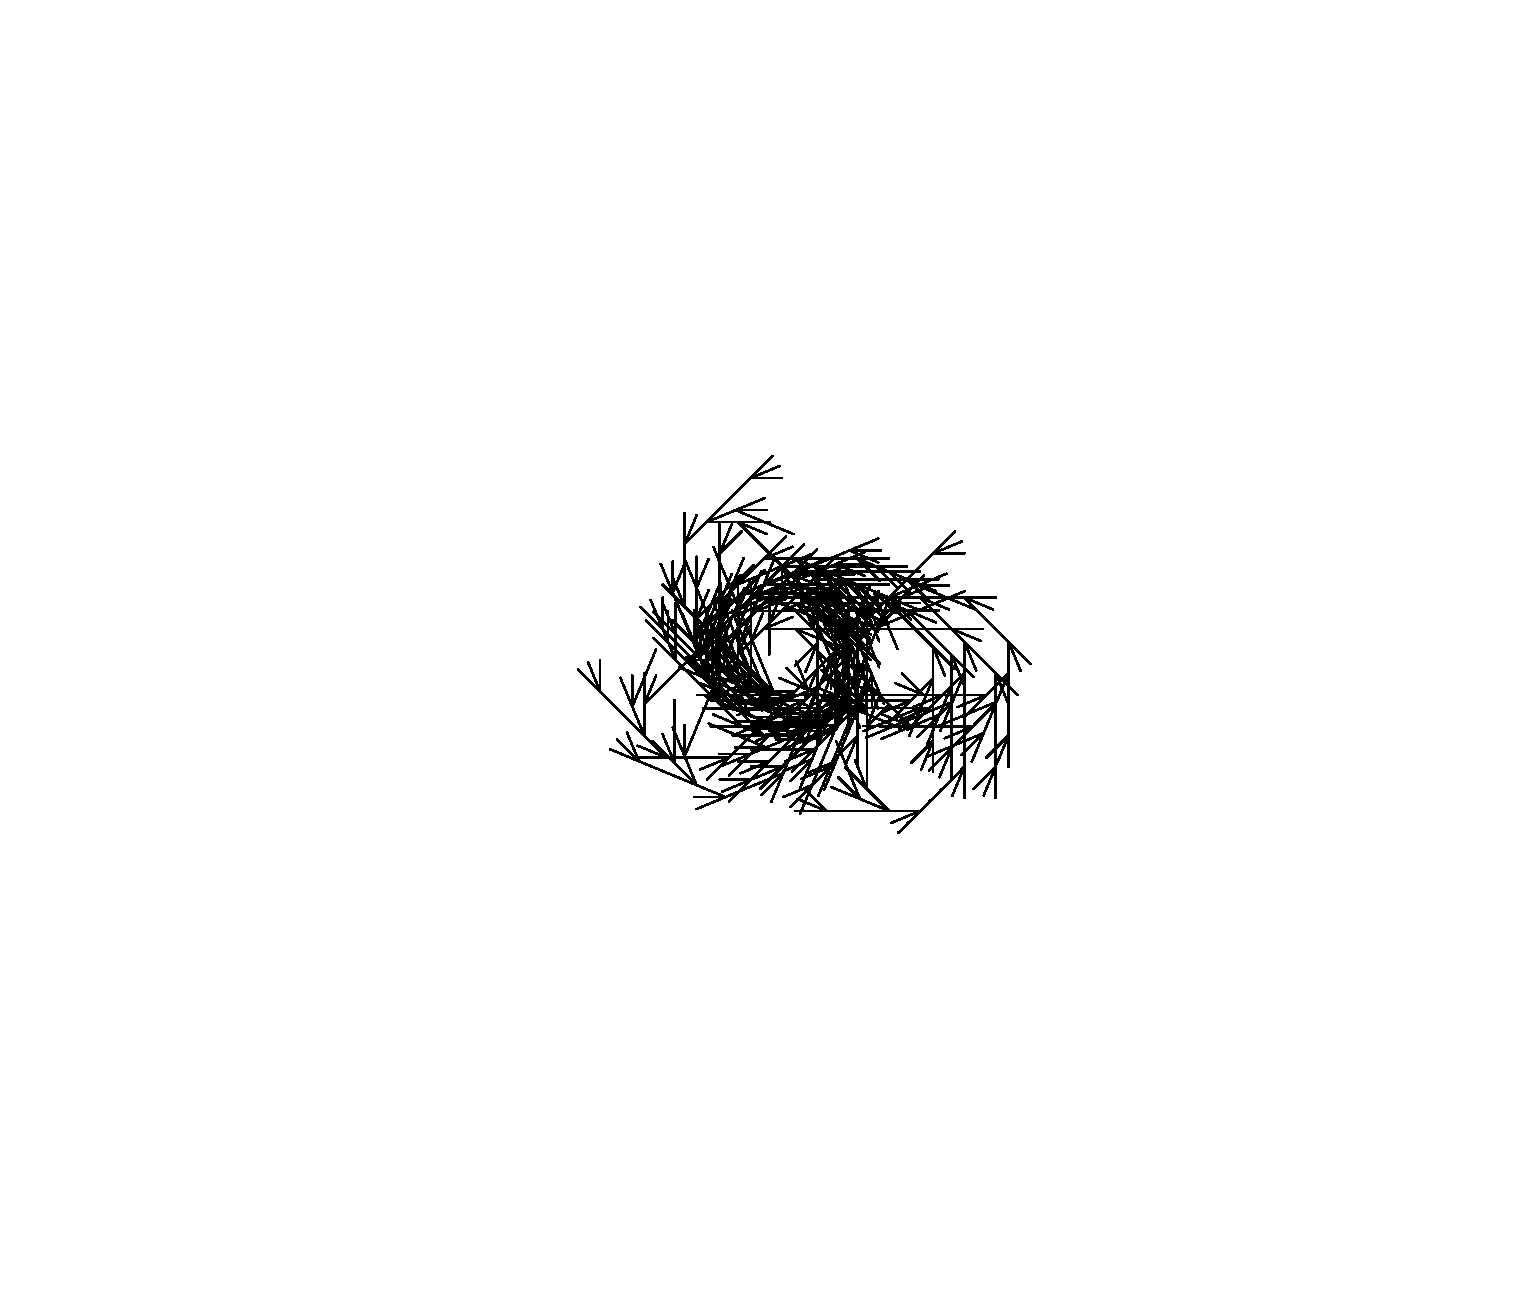
\includegraphics[width=.5\textwidth]{LSystem/plant_1} &
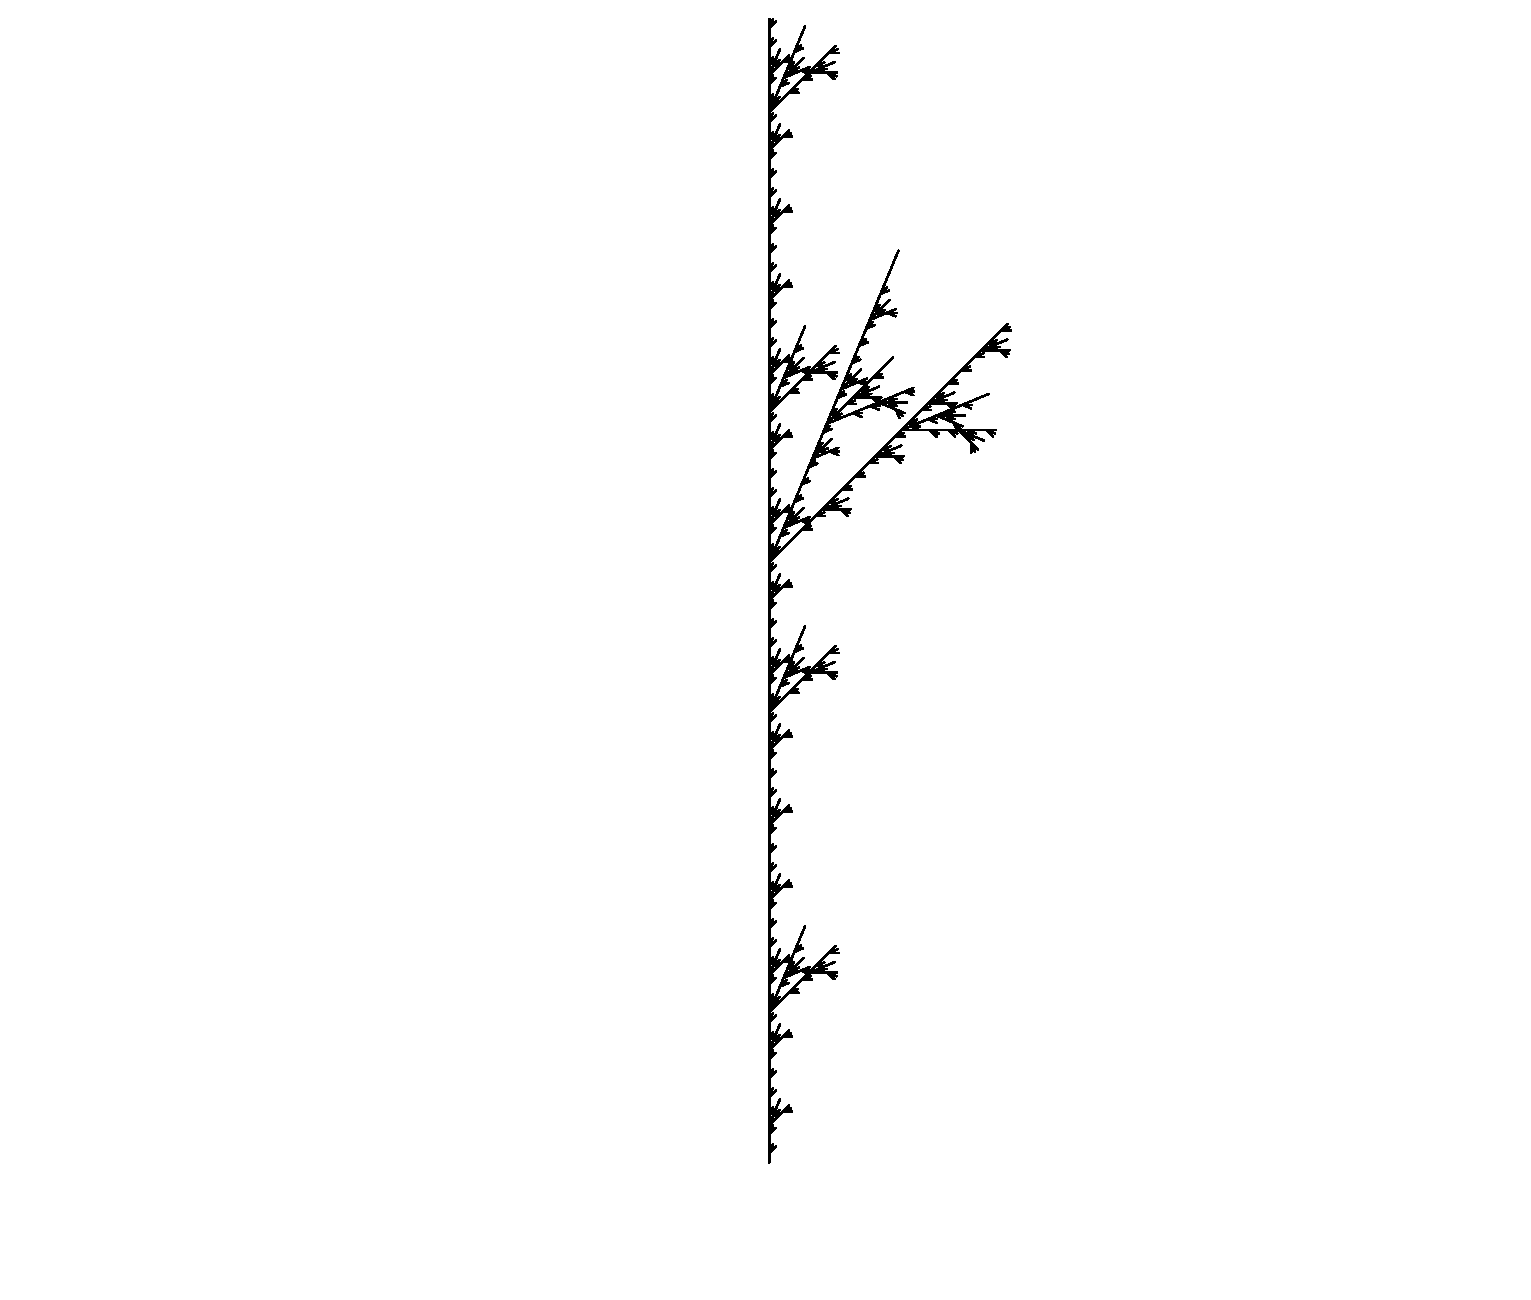
\includegraphics[width=.5\textwidth]{LSystem/plant_2} \\
Symmetrical G & Symmetrical G with +/- swapping \\


\includegraphics[width=.5\textwidth]{LSystem/plant_3} &
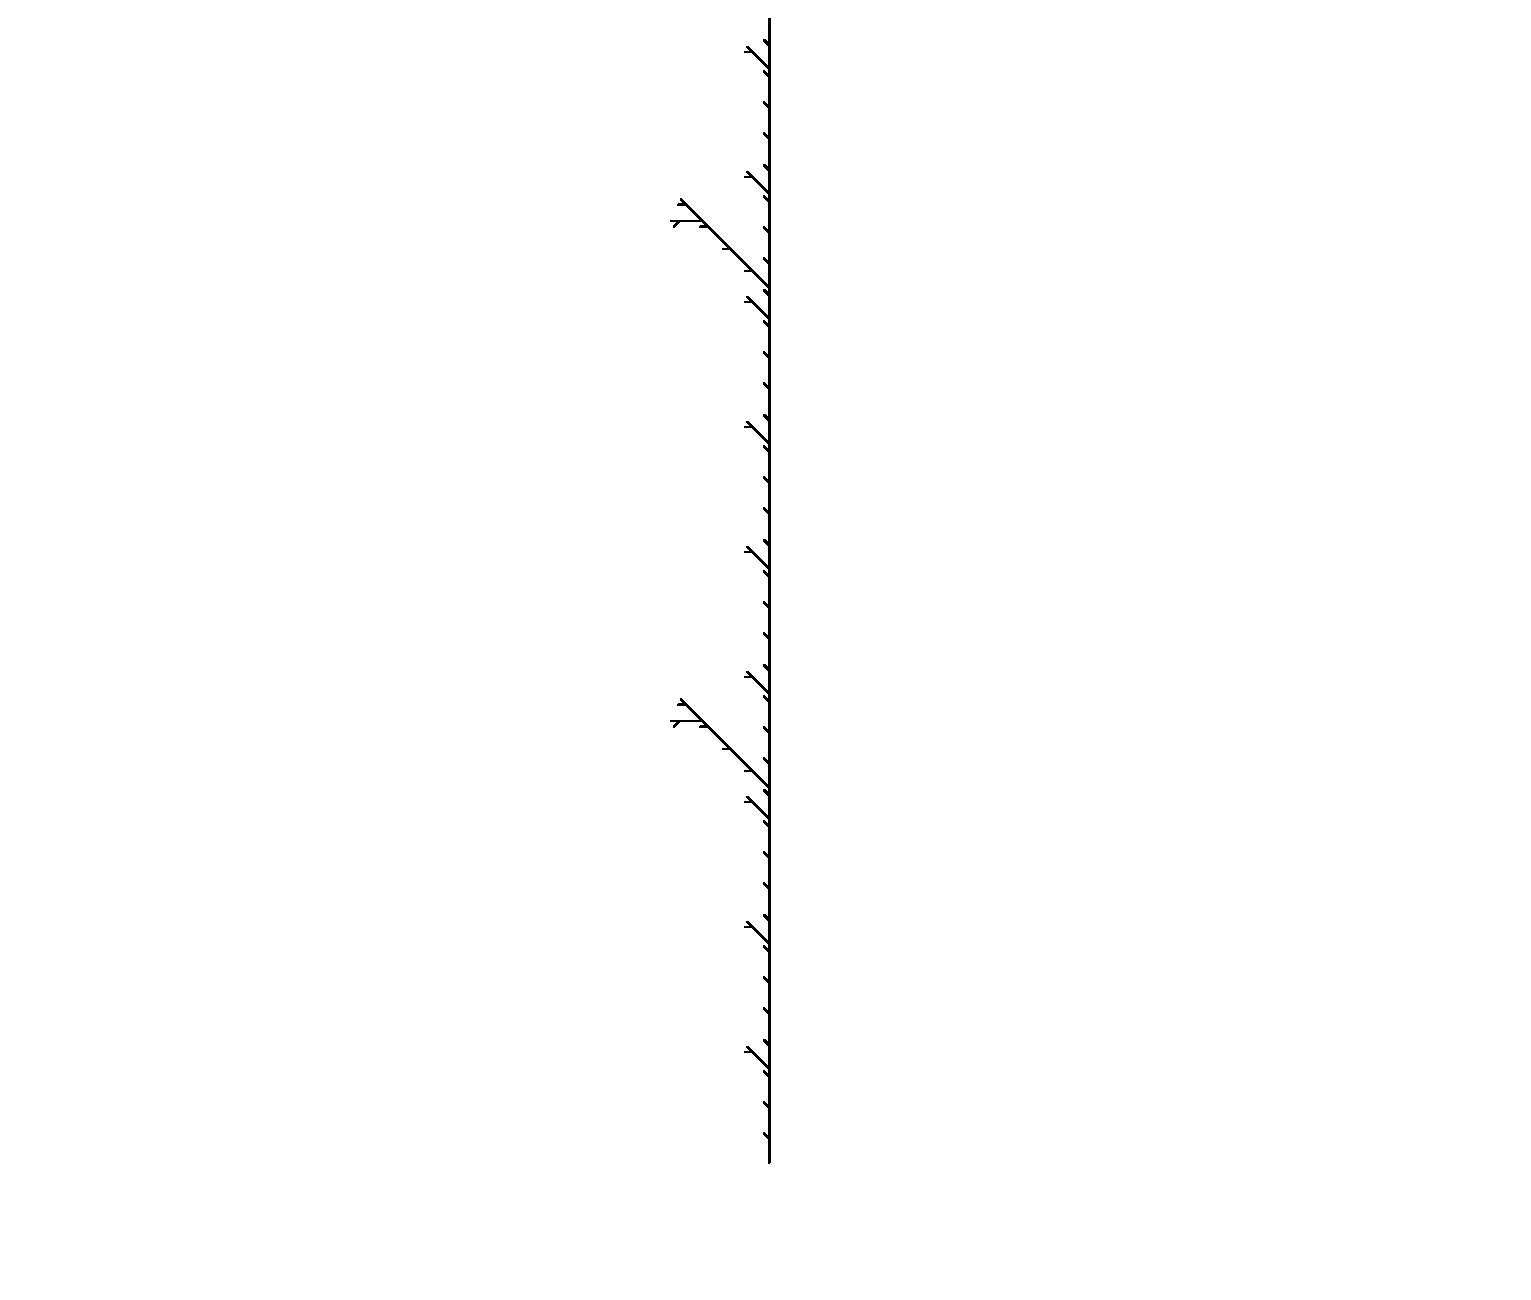
\includegraphics[width=.5\textwidth]{LSystem/plant_4} \\
Symmetrical F only & Symmetrical F only with +/- swapping
\end{tabular}

\begin{tabular}{ c c }
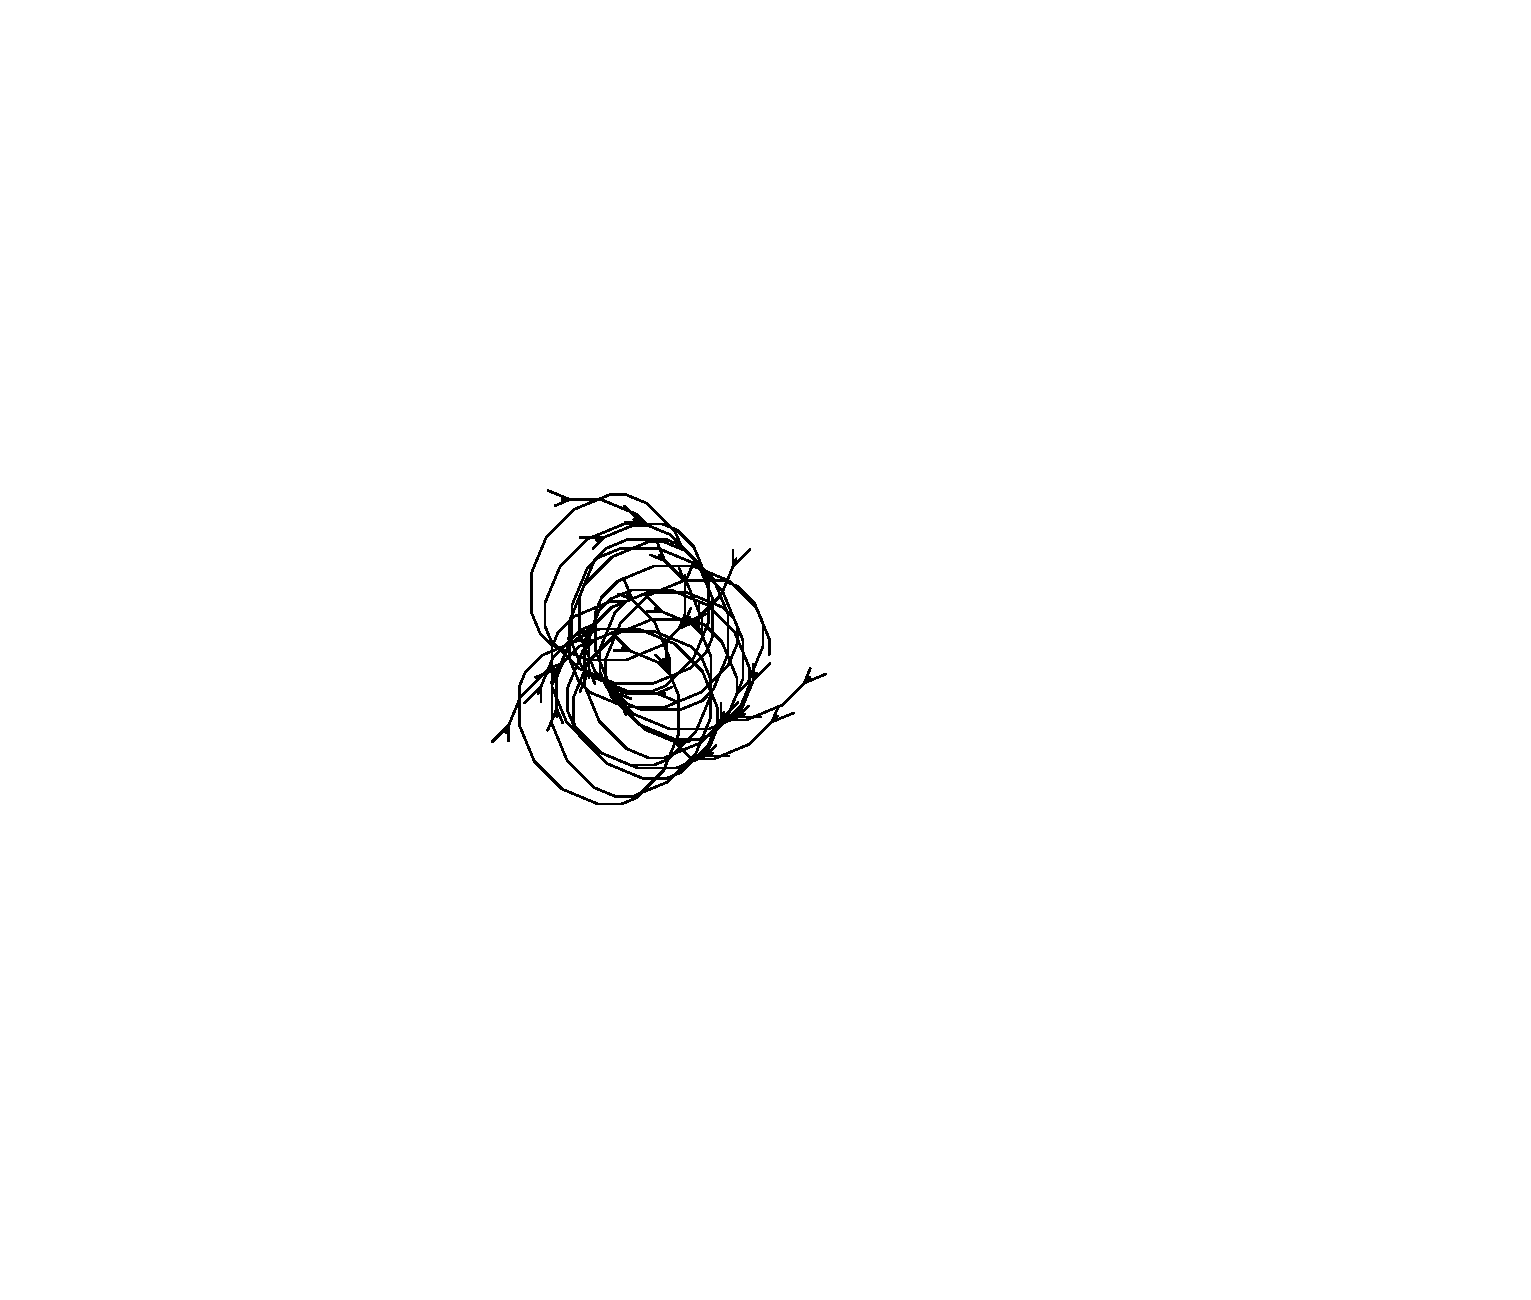
\includegraphics[width=.5\textwidth]{LSystem/plant_5} &
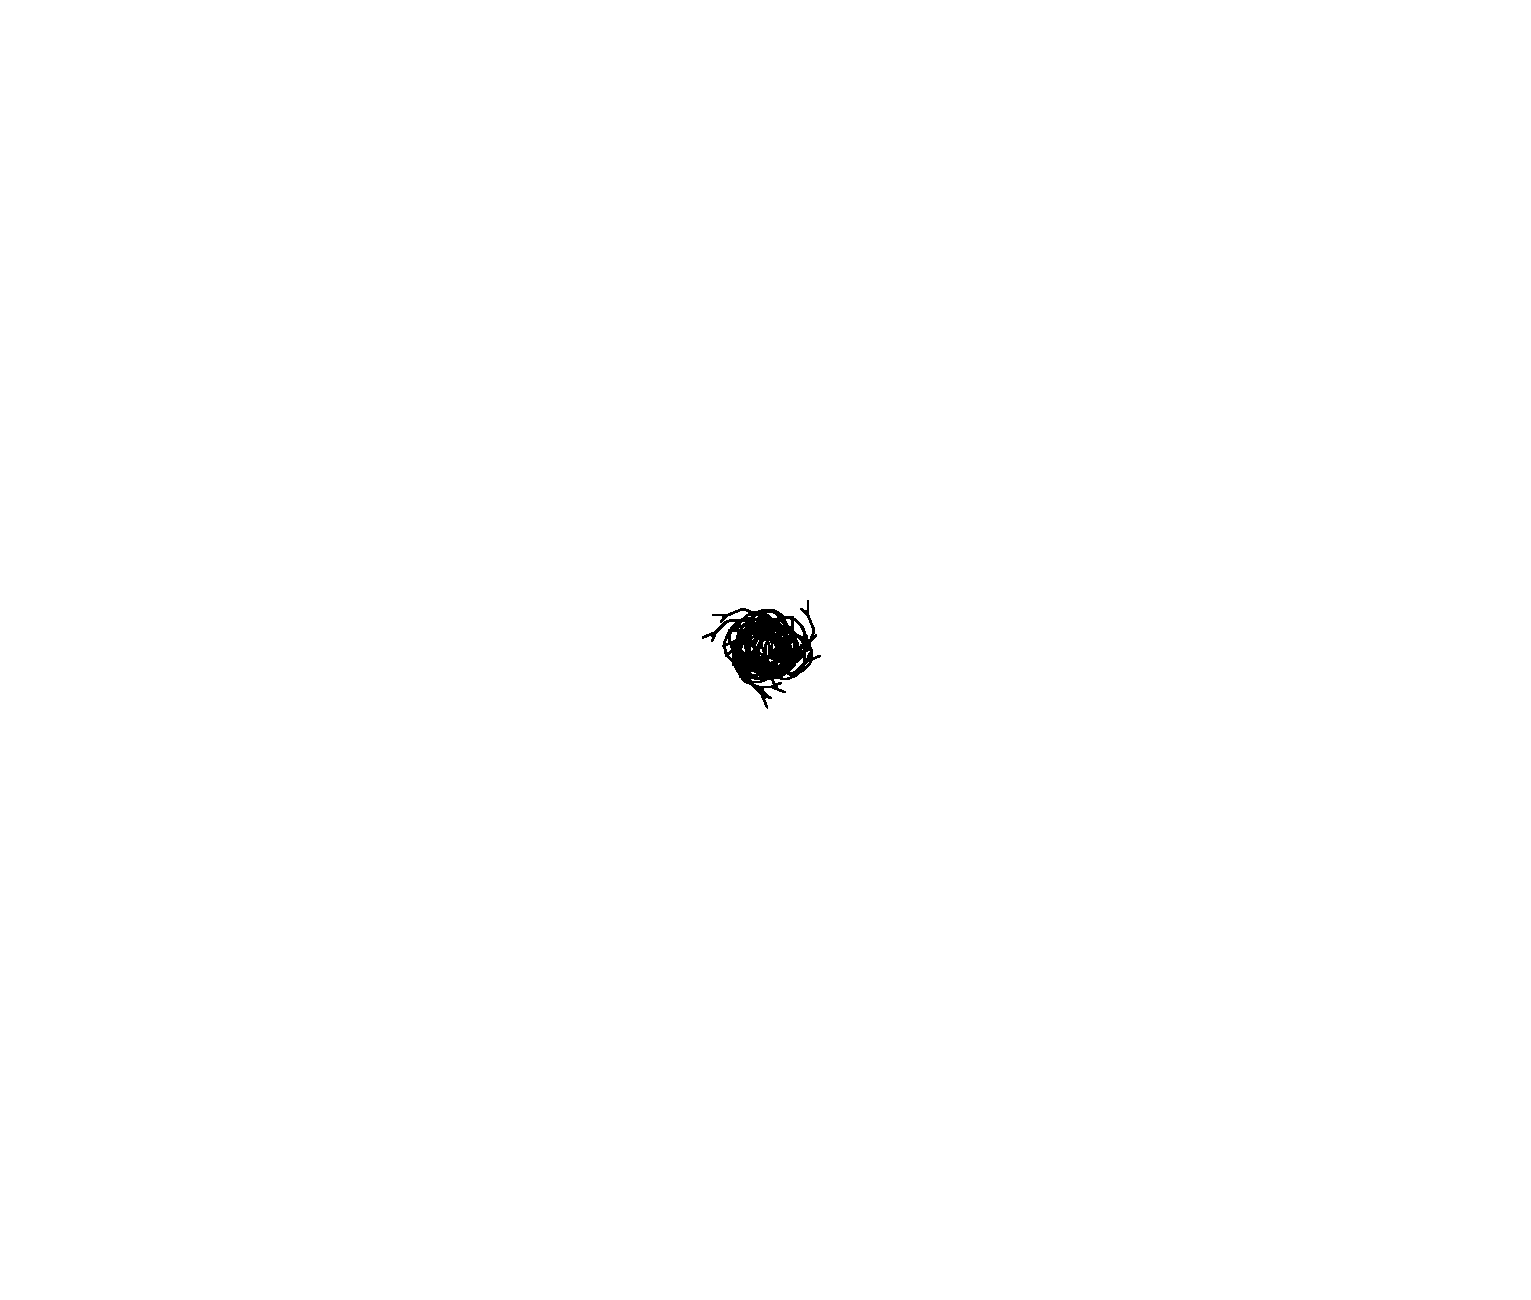
\includegraphics[width=.5\textwidth]{LSystem/plant_6} \\
Turning F & Symmetrical Turning F \\

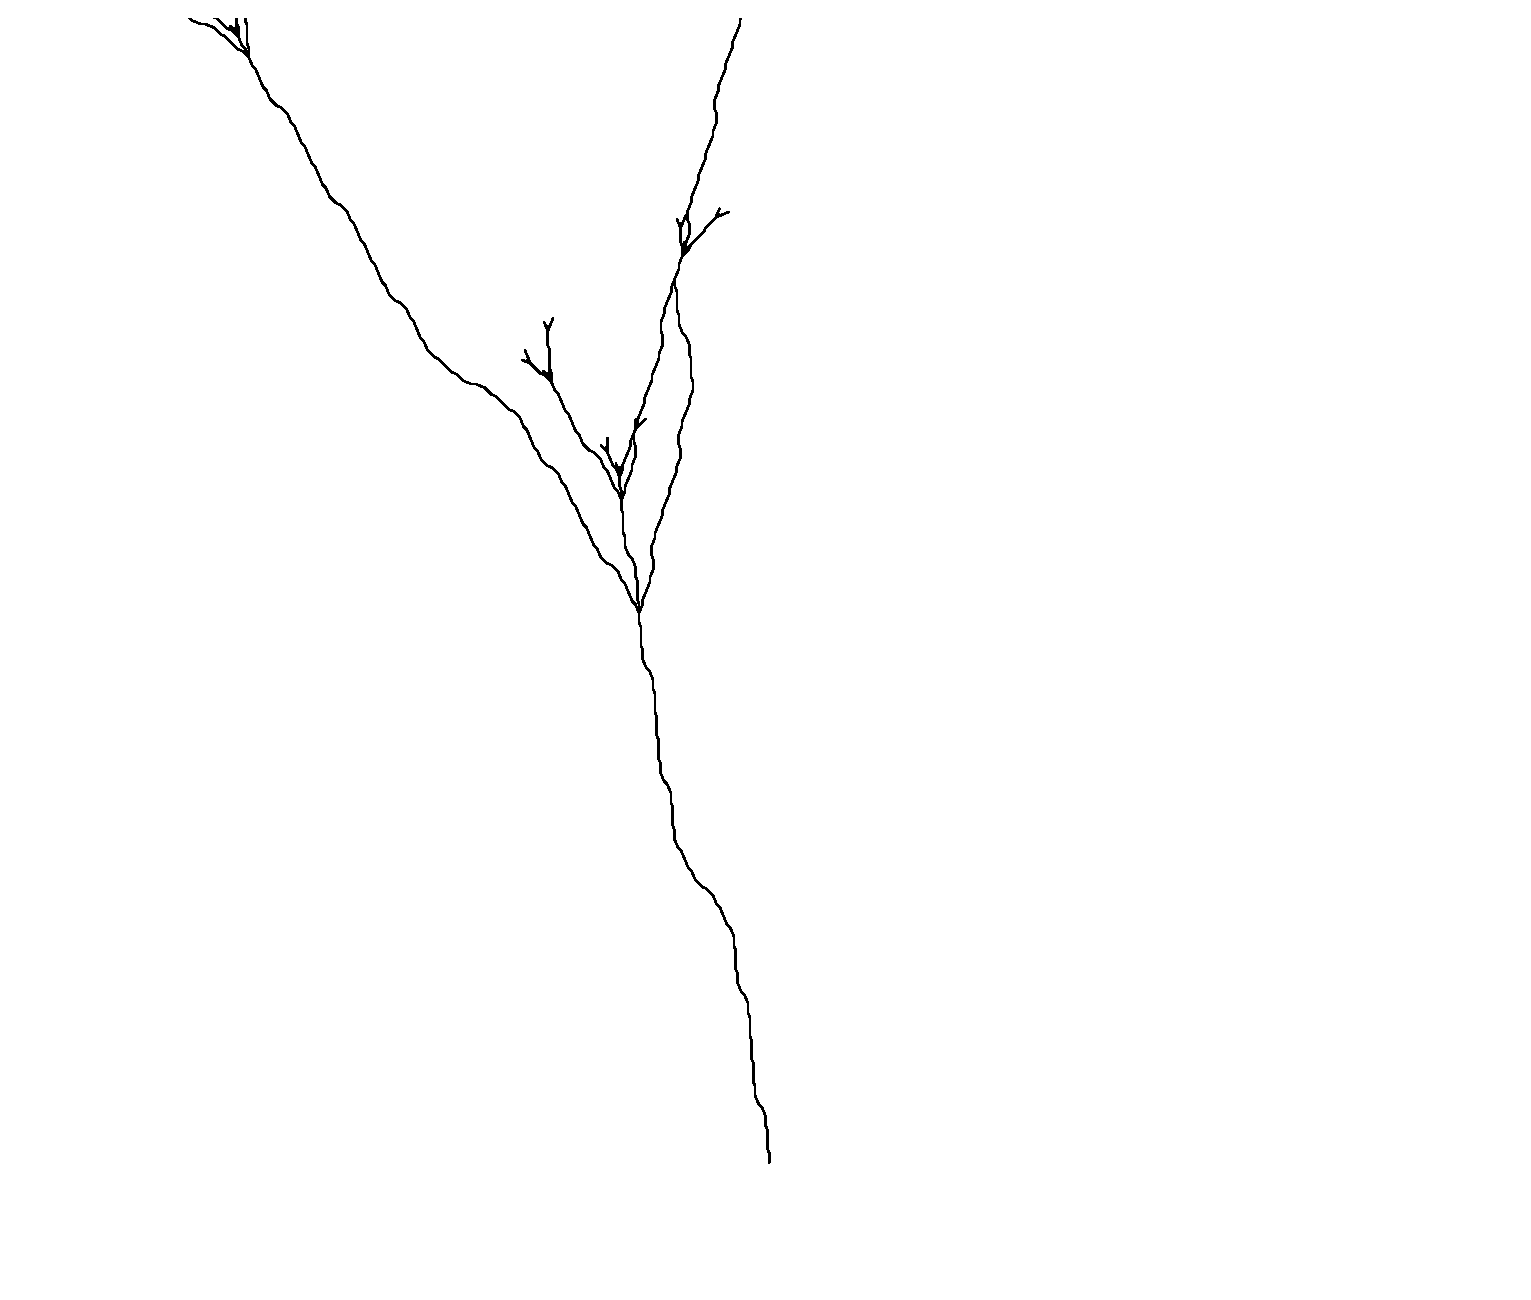
\includegraphics[width=.5\textwidth]{LSystem/plant_7} &
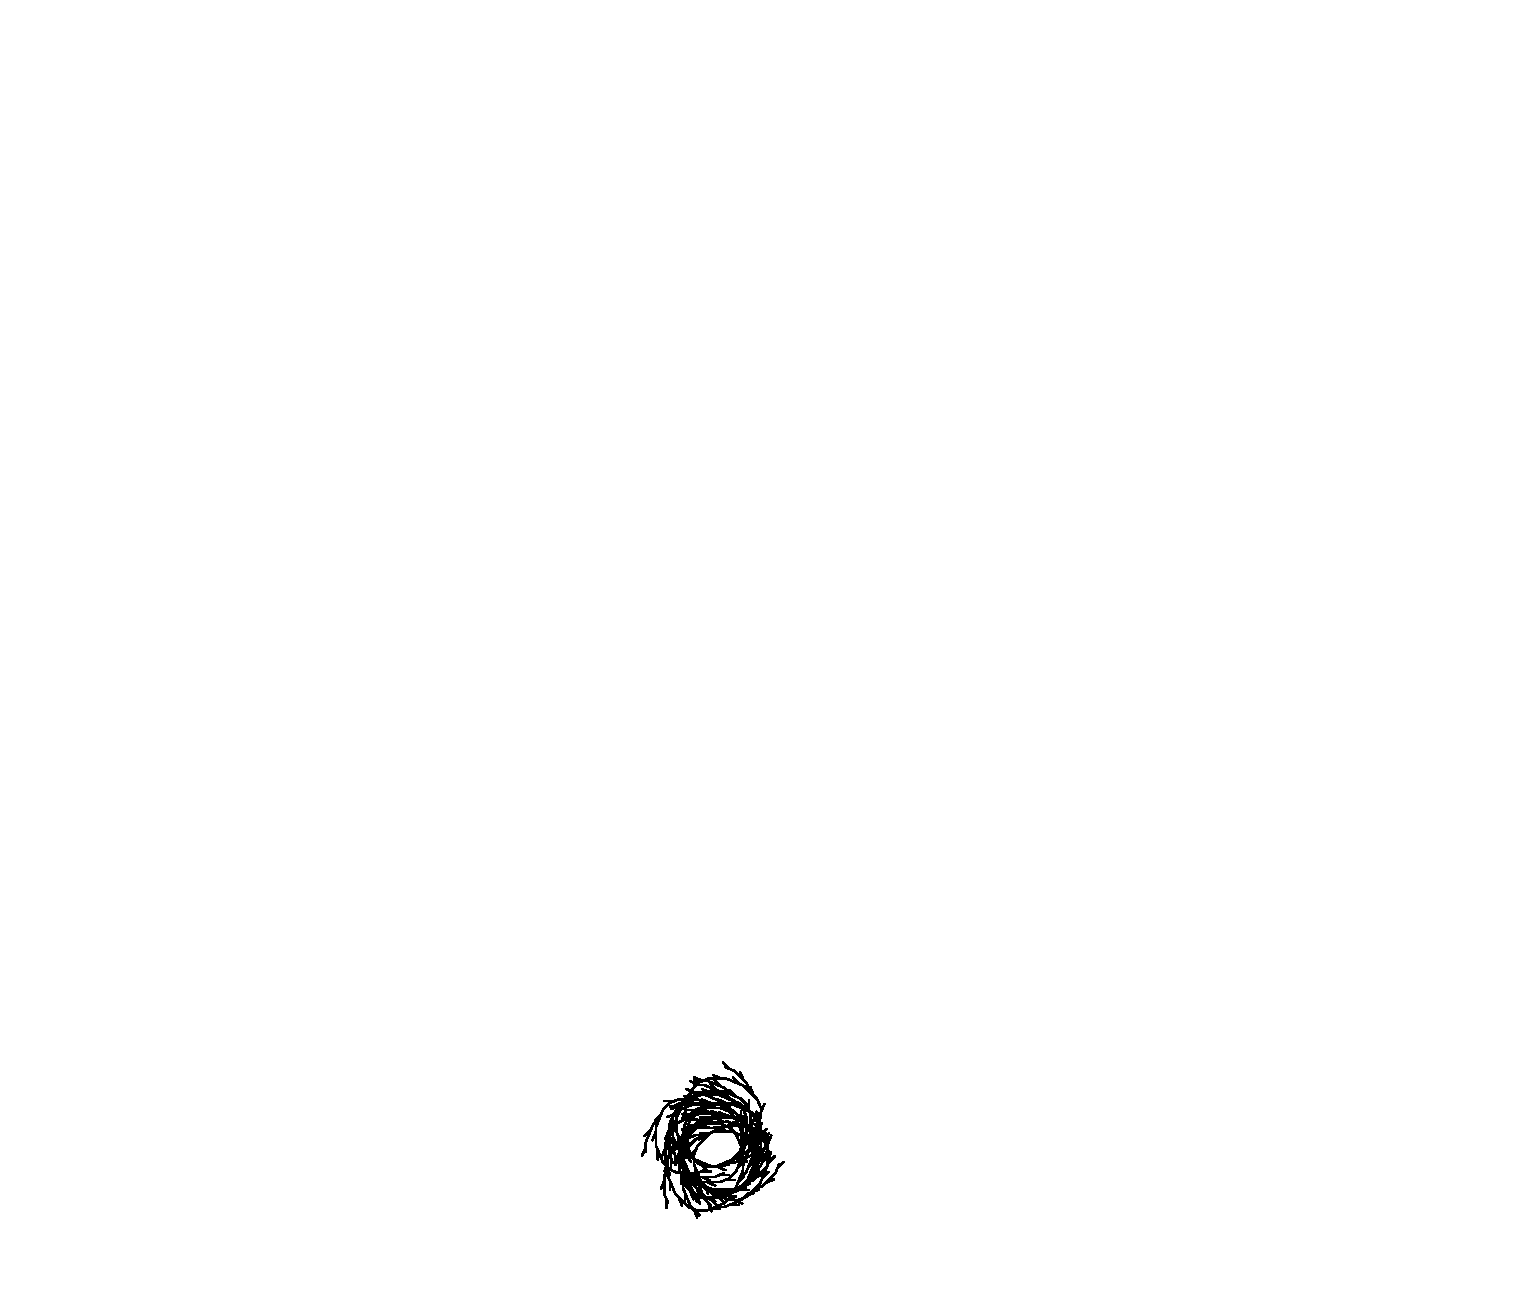
\includegraphics[width=.5\textwidth]{LSystem/plant_8} \\
Symmetrical Turning F with +/- swapping & Similar G \& F
\end{tabular}

\begin{tabular}{ c c c }
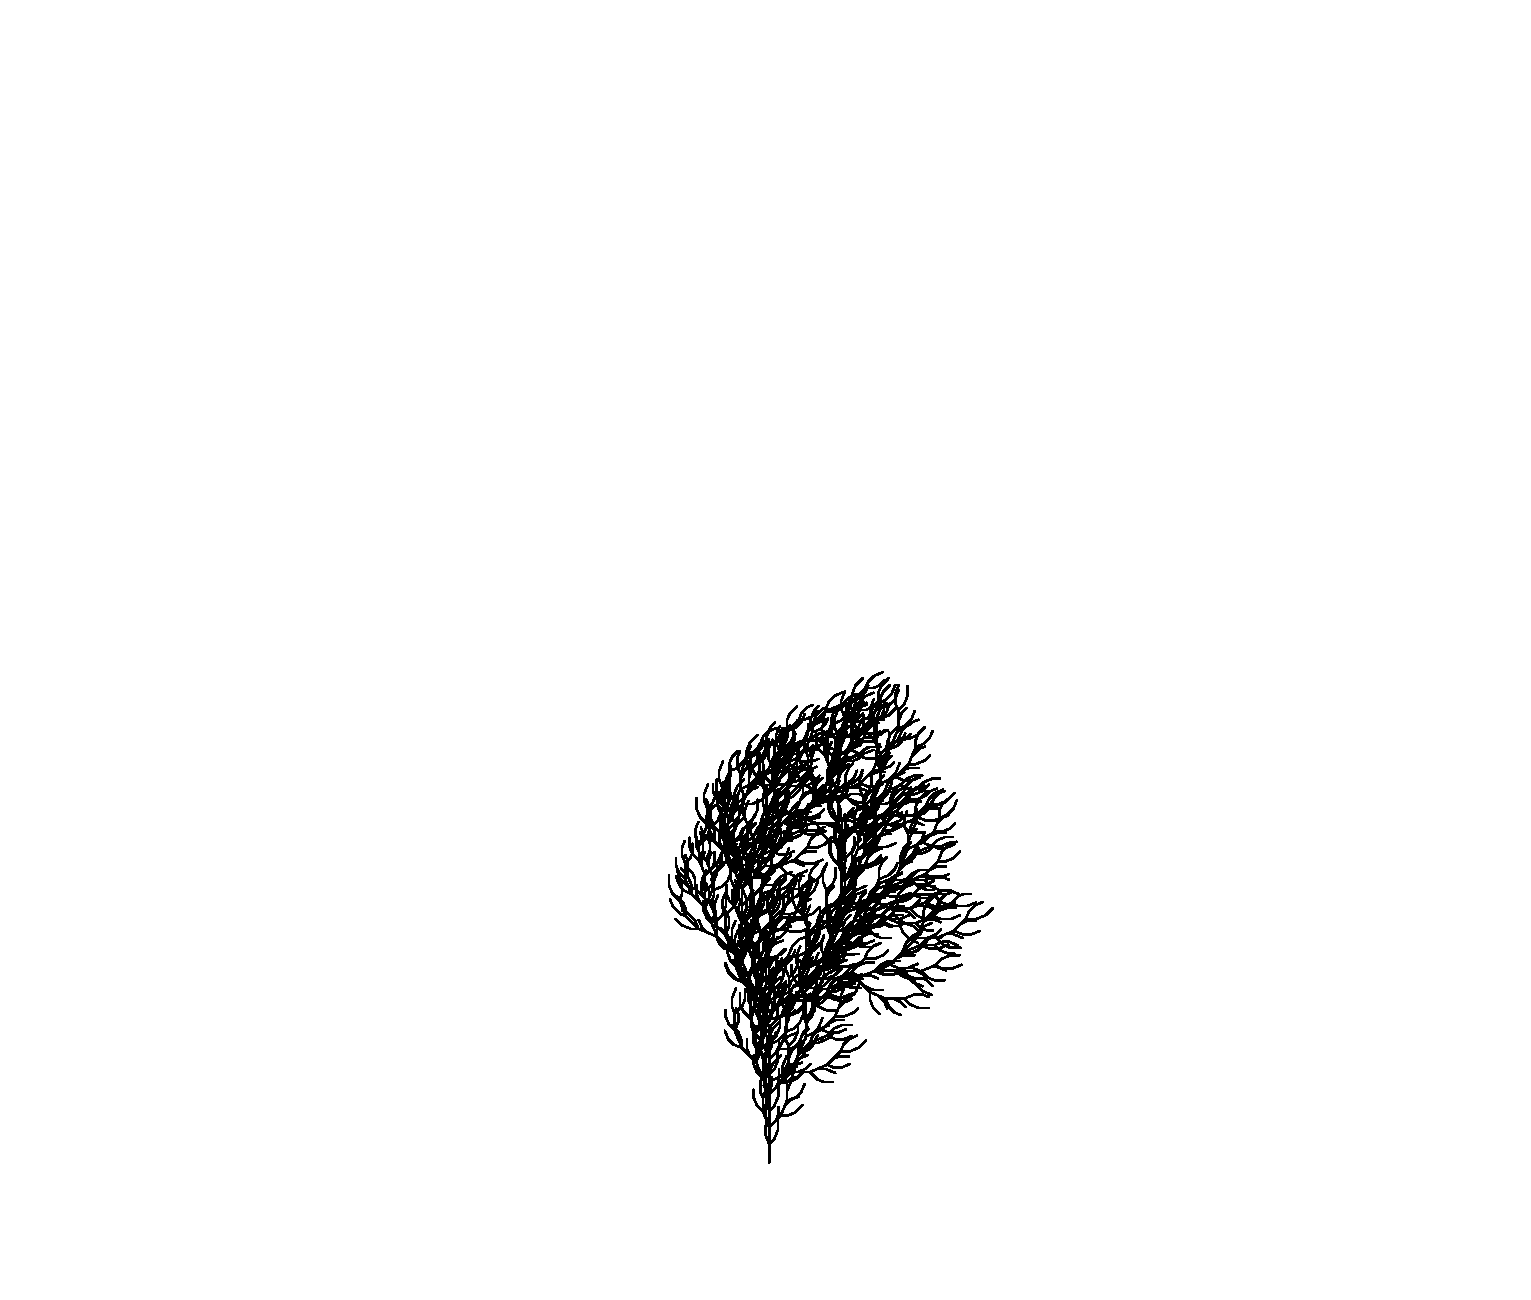
\includegraphics[width=.3\textwidth]{LSystem/plant_9} &
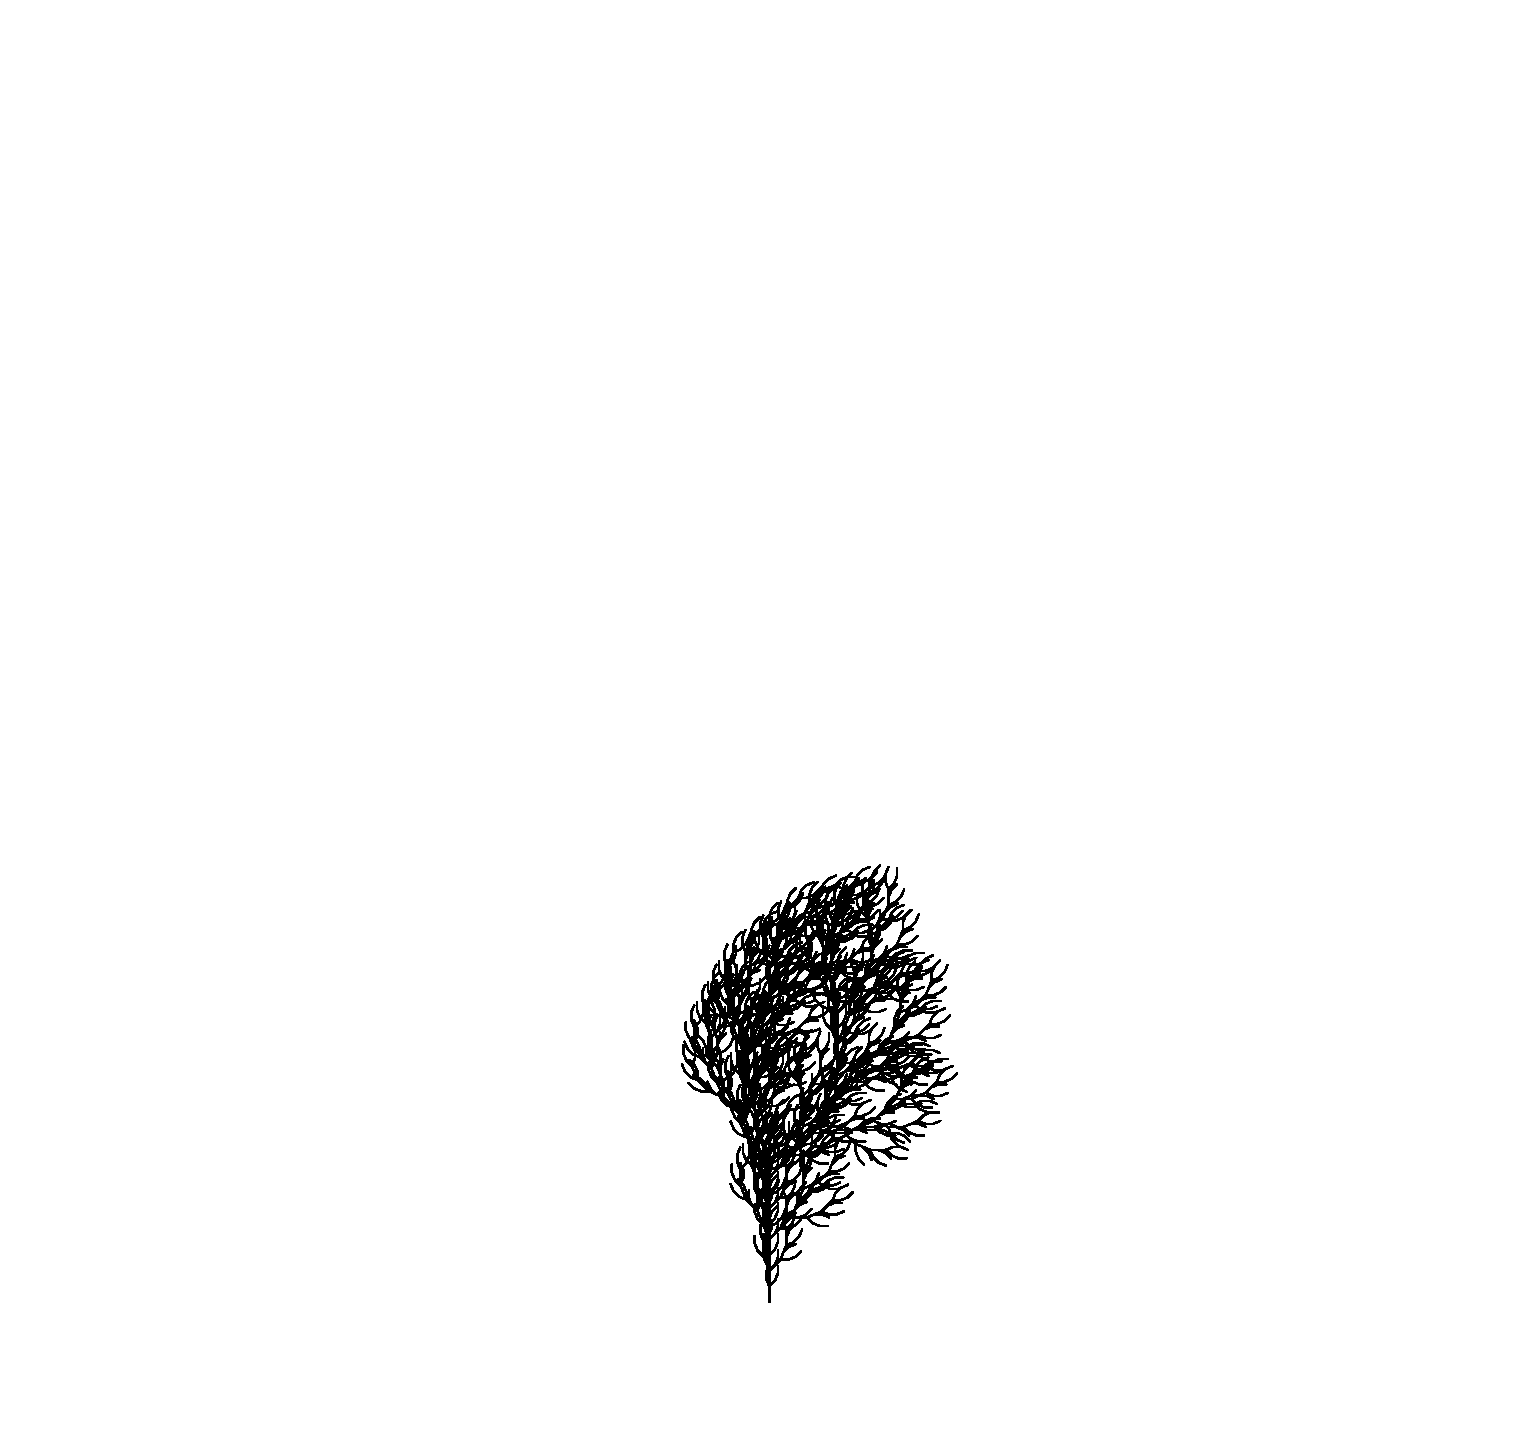
\includegraphics[width=.3\textwidth]{LSystem/lsystem_b} &
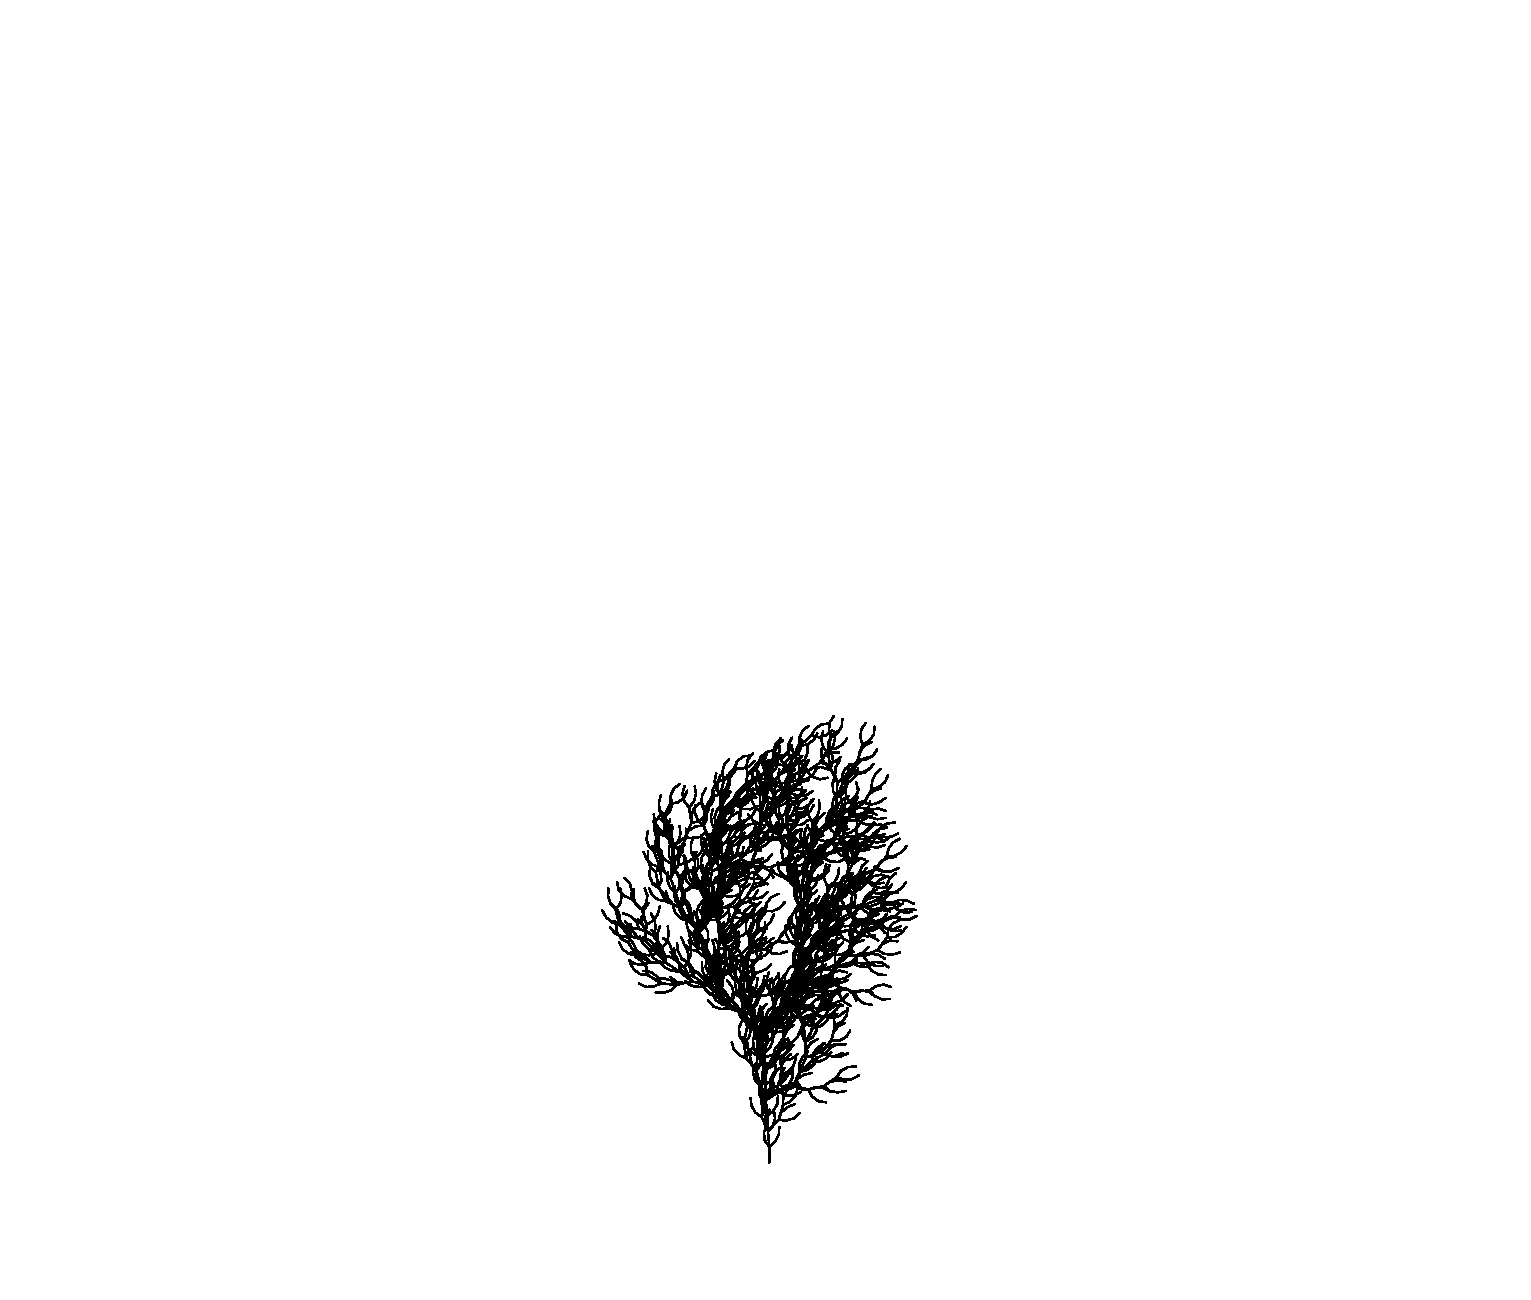
\includegraphics[width=.3\textwidth]{LSystem/plant_10} \\
Randomized distance (d) & 7.24(b) for comparison & Randomized turn ($\delta$)
\end{tabular}

\newpage
\section{RIFS Results} \label{RIFS_results}
\begin{tabular}{ c c }
\includegraphics[width=.5\textwidth]{RIFS/rifs_sierpinski} &
\includegraphics[width=.5\textwidth]{RIFS/rifs_square} \\
Sierpinski Gasket & Square \\
\includegraphics[width=.5\textwidth]{RIFS/rifs_barnsleyfern} &
\includegraphics[width=.5\textwidth]{RIFS/rifs_tree} \\
Barnsley Fern\footnote{I'm pretty sure the one in the book was rotated after it was generated to make it look more like a fern.} & Tree
\end{tabular}